\documentclass[11pt, a4paper]{article}

% --- Packages ---
\usepackage[a4paper, top=2.5cm, bottom=2.5cm, left=2.5cm, right=2.5cm]{geometry}
\usepackage{amsmath, amssymb}
\usepackage{tikz}
\usetikzlibrary{shapes.geometric, arrows.meta, positioning}
\usepackage{booktabs}
\usepackage{parskip}
\usepackage{microtype}
\usepackage{fancyhdr}
\usepackage{titlesec}
\usepackage{xcolor}
\usepackage{mdframed}
\usepackage{enumitem}
\usepackage{hyperref}

\hypersetup{colorlinks=true, linkcolor=black, urlcolor=blue}

% --- Page style ---
\pagestyle{fancy}
\fancyhf{}
\renewcommand{\headrulewidth}{0.4pt}
\renewcommand{\footrulewidth}{0.4pt}
\fancyhead[L]{\small\textit{Study Notes: Damage Propagation Modeling}}
\fancyhead[R]{\small\thepage}
\fancyfoot[C]{\small\textit{``I'm not stupid, I'm just slow''}}

% --- Section style ---
\titleformat{\section}{\large\bfseries}{}{0em}{}[\titlerule]
\titleformat{\subsection}{\normalsize\bfseries}{}{0em}{}

% --- Highlight box ---
\newmdenv[
  backgroundcolor=gray!10,
  linecolor=gray!50,
  linewidth=0.8pt,
  innerleftmargin=10pt,
  innerrightmargin=10pt,
  innertopmargin=8pt,
  innerbottommargin=8pt,
  skipabove=8pt,
  skipbelow=8pt
]{keybox}

% --- TikZ styles ---
\tikzset{
  block/.style={
    rectangle, rounded corners=4pt,
    minimum width=2.6cm, minimum height=0.9cm,
    text centered, text width=2.4cm,
    draw=black!70, fill=gray!12,
    font=\small
  },
  decision/.style={
    diamond, aspect=2.2,
    minimum width=2.8cm, minimum height=0.9cm,
    text centered, text width=2.4cm,
    draw=black!70, fill=gray!20,
    font=\small
  },
  arrow/.style={-{Stealth[length=5pt]}, thick, black!70}
}

% -------------------------------------------------------------------
\begin{document}
% -------------------------------------------------------------------

{\Large\bfseries Reading Notes: Damage Propagation Modeling\\
for Aircraft Engine Run-to-Failure Simulation}

\smallskip
{\small Saxena, Goebel, Simon, Eklund --- PHM'08}

\medskip\hrule\bigskip

% -------------------------------------------------------------------
\section{The Problem Being Solved}
% -------------------------------------------------------------------

Anyone who wants to build a machine learning model that predicts
\textbf{when an aircraft engine will fail} faces an immediate obstacle:
\emph{where does the training data come from?}

Real engines do not conveniently fail on schedule. Fleet operators who do
accumulate run-to-failure records tend to keep them private for competitive
reasons. What little public data exists is scarce and inconsistent, making
it impossible for researchers to fairly compare their algorithms.

\begin{keybox}
\textbf{Core question the paper answers:}
Can we simulate realistic engine degradation data that is
``good enough'' to train and benchmark prognostics algorithms?
\end{keybox}

The answer is yes --- by combining a physics-based engine simulator with
a simple but plausible damage model.

% -------------------------------------------------------------------
\section{The Tool: C-MAPSS}
% -------------------------------------------------------------------

\textbf{C-MAPSS} (Commercial Modular Aero-Propulsion System Simulation)
is a NASA MATLAB/Simulink model of a large commercial turbofan engine
(90,000\,lb thrust class). It is the ``test bench'' of this paper.

The engine has five rotating components the simulation can degrade
independently: \textbf{Fan}, \textbf{LPC}, \textbf{HPC}, \textbf{HPT},
and \textbf{LPT}.

For each component, two health-related parameters can be adjusted:
\begin{itemize}[noitemsep]
  \item \textbf{Efficiency modifier} --- how efficiently the component
        converts energy
  \item \textbf{Flow modifier} --- how much air mass passes through it
\end{itemize}

Reducing these values simulates wear and deterioration.
The simulation then produces 21 sensor readings per time step ---
temperatures, pressures, speeds, and ratios --- the same kind of data
a real engine health monitoring system would record.

For the competition dataset, only \textbf{HPC degradation} was simulated.
The other four components were left healthy intentionally, to keep the
challenge focused.

% -------------------------------------------------------------------
\section{How Damage Was Injected}
% -------------------------------------------------------------------

\subsection{Why exponential?}

Real degradation in mechanical components tends to start slowly and
accelerate over time --- think of a crack that grows faster the longer it
exists. An \textbf{exponential} function captures this macro-level
behaviour simply, without needing to model microscopic physics.

\subsection{The health equation}

For each component, efficiency $e(t)$ and flow $f(t)$ are each described
by the same form:

\begin{equation}
  h(t) \;=\; 1 - d - \exp\!\left\{a\,t^{b}\right\}
  \label{eq:health}
\end{equation}

Reading each term:

\begin{center}
\begin{tabular}{@{}lp{9cm}@{}}
  \toprule
  Term & Meaning \\
  \midrule
  $h(t)$   & Health value at cycle $t$. Starts near 1, drifts toward 0. \\
  $d$      & Initial deterioration. Every engine starts with a tiny
             random amount of wear (manufacturing variation). \\
  $a$      & Rate of degradation. Randomly chosen per engine within
             $[0.001,\, 0.003]$. Governs how fast things get worse. \\
  $b$      & Shape exponent, chosen in $[1.4,\, 1.6]$.
             Makes the decay curve slightly super-exponential. \\
  $t$      & Time in engine cycles (one flight $\approx$ one cycle). \\
  \bottomrule
\end{tabular}
\end{center}

\medskip
Both efficiency and flow get their own copy of this equation (with their
own $a$, $b$, $d$ values), drawn randomly for each simulated engine unit.
This is what makes every engine life in the dataset different.

% -------------------------------------------------------------------
\section{How Failure Was Defined}
% -------------------------------------------------------------------

\subsection{The health index}

The engine does not ``break'' suddenly. Instead, failure is defined as
the moment when the engine can no longer operate safely within its
design limits. Four safety margins are tracked continuously:

\begin{itemize}[noitemsep]
  \item Fan stall margin
  \item LPC stall margin
  \item HPC stall margin
  \item EGT (exhaust gas temperature) margin
\end{itemize}

Each margin is normalised to $[0, 1]$. The overall
\textbf{health index} $H(t)$ is the \emph{minimum} of all four:

\begin{equation}
  H(t) \;=\; \min\!\bigl(m_\text{Fan},\; m_\text{HPC},\;
                          m_\text{LPC},\; m_\text{EGT}\bigr)
  \label{eq:hindex}
\end{equation}

Whichever margin runs out first determines the end of life.
The simulation stops when $H(t) = 0$.

\begin{keybox}
\textbf{Intuition:} Think of $H(t)$ as ``how much safety buffer
is left.'' When any one buffer hits zero --- whether from stall risk
or overheating --- the engine has reached its operational limit.
The competition participants never see this index directly;
they must infer it from the sensor readings.
\end{keybox}

% -------------------------------------------------------------------
\section{The Simulation Pipeline}
% -------------------------------------------------------------------

\begin{center}
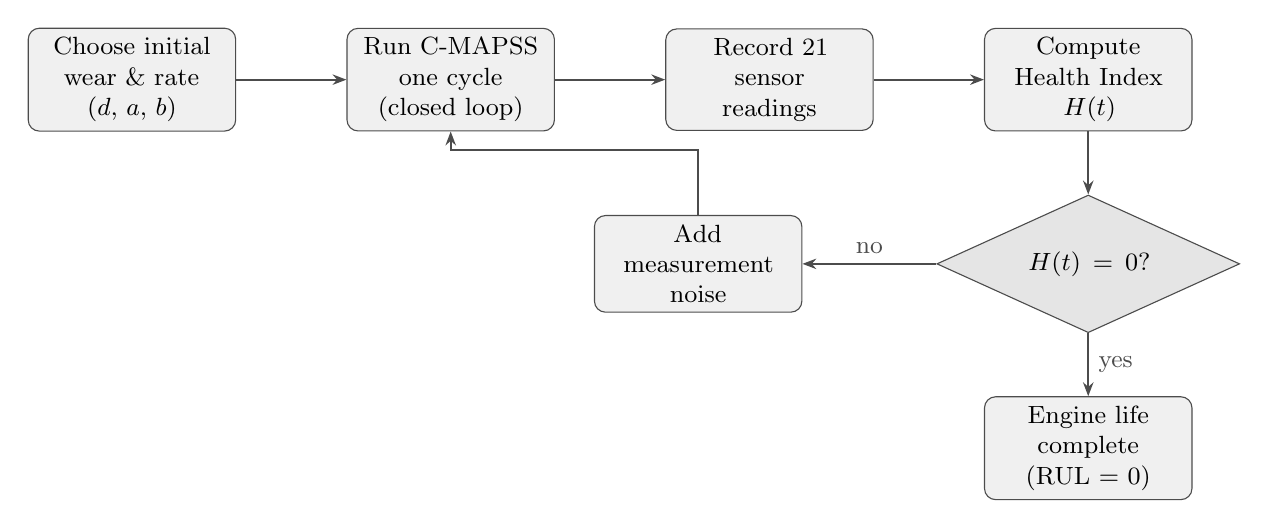
\begin{tikzpicture}[node distance=0.55cm and 1.4cm]

  \node[block] (init) {Choose initial\\wear \& rate\\($d$, $a$, $b$)};

  \node[block, right=of init] (cmapss) {Run C-MAPSS\\one cycle\\(closed loop)};

  \node[block, right=of cmapss] (sensor) {Record 21\\sensor\\readings};

  \node[block, right=of sensor] (hindex) {Compute\\Health Index\\$H(t)$};

  \node[decision, below=0.8cm of hindex] (check) {$H(t) = 0$?};

  \node[block, left=of check, xshift=-0.3cm] (noise) {Add\\measurement\\noise};

  \node[block, below=0.8cm of check] (done) {Engine life\\complete\\(RUL = 0)};

  \draw[arrow] (init) -- (cmapss);
  \draw[arrow] (cmapss) -- (sensor);
  \draw[arrow] (sensor) -- (hindex);
  \draw[arrow] (hindex) -- (check);
  \draw[arrow] (check) -- node[right]{\small yes} (done);
  \draw[arrow] (check) -- node[above]{\small no} (noise);
  \draw[arrow] (noise) -- ++(0, 1.45) -| (cmapss);

\end{tikzpicture}
\end{center}

This loop is run once per simulated engine. Hundreds of independent
engine lives were generated, each with different random parameters,
to form the final dataset.

% -------------------------------------------------------------------
\section{Realism: Noise and Initial Wear}
% -------------------------------------------------------------------

Two features make the data harder to work with --- intentionally,
to match real conditions.

\textbf{Initial wear.} Every engine starts with a tiny random degradation
(up to 1\%) simulating manufacturing imperfection. No two engines
begin at exactly the same health state.

\textbf{Noise.} Three noise layers are stacked:
\begin{enumerate}[noitemsep]
  \item Random degradation rate parameters ($a_k$, $b_k$) per engine
  \item Process noise through the simulation (e.g.\ maintenance effects)
  \item Measurement noise added directly to sensor outputs
\end{enumerate}

The process noise is a \emph{mixture} of two distributions with
different variances, making it harder to characterise than simple
Gaussian noise. This is why the efficiency trajectory in the paper
is not monotonically decreasing --- small recoveries between flights
are possible, just as real maintenance can partially restore performance.

% -------------------------------------------------------------------
\section{How Performance Was Measured}
% -------------------------------------------------------------------

The competition task was: given sensor readings up to some cycle,
predict how many cycles remain (\textbf{Remaining Useful Life, RUL}).

The scoring function is \textbf{asymmetric}:

\begin{equation}
  s \;=\; \begin{cases}
    \displaystyle\sum_{i=1}^{n} e^{-d/10} - 1
      & \text{if } d < 0 \quad \text{(predicted early)} \\[8pt]
    \displaystyle\sum_{i=1}^{n} e^{\,d/13} - 1
      & \text{if } d \geq 0 \quad \text{(predicted late)}
  \end{cases}
  \label{eq:score}
\end{equation}

where $d = \hat{t}_\text{RUL} - t_\text{RUL}$ (estimated minus true RUL).

\begin{keybox}
\textbf{Why asymmetric?}
Predicting \emph{too late} is more dangerous than predicting
\emph{too early}. A late prediction means the engine might fly past
its safe limit. An early prediction means unnecessary maintenance ---
costly, but not catastrophic. The denominator 13 (late penalty)
is larger than 10 (early penalty), so the exponential grows faster
for late predictions.
\end{keybox}

% -------------------------------------------------------------------
\section{Summary: What This Paper Gives Us}
% -------------------------------------------------------------------

\begin{center}
\begin{tabular}{@{}lp{9cm}@{}}
  \toprule
  Contribution & What it means in practice \\
  \midrule
  C-MAPSS simulation  & A physics-grounded engine model anyone can use \\
  Exponential damage model & A simple, realistic way to simulate wear \\
  Health index definition & A principled failure criterion \\
  Noise strategy & Realistic, non-trivial sensor data \\
  Asymmetric scoring & A metric that reflects aviation safety priorities \\
  Public dataset & A common benchmark for comparing RUL algorithms \\
  \bottomrule
\end{tabular}
\end{center}

\bigskip
The paper is essentially the \textbf{methodology report} that accompanies
the dataset. Understanding it is the prerequisite for working with
C-MAPSS data intelligently --- knowing not just what the numbers are,
but where they came from and what assumptions went into them.

% -------------------------------------------------------------------
\end{document}
